\section{Resultados y análisis}

\subsection{Tabla de pruebas}
La Tabla~\ref{tab:pruebas} resume las cuatro condiciones con los valores exactos y las métricas medidas a partir de los datos exportados por GNU Radio (200\,000 bits por prueba). La potencia de ruido medida ($\sigma^2=0{,}010$) confirma \texttt{noise\_amp}$=0{,}10$, equivalente a $E_b/N_0\approx29$~dB respecto al camino directo. La potencia recibida coincide con $1+|\alpha|^2+2|\alpha|\rho_1+\sigma^2$ con error menor de $10^{-3}$. El término $\rho_1$ es la autocorrelación de la secuencia de prueba (la fuente del curso repite 1000 bits) y vale entre $-0{,}056$ y $0{,}064$ según la ejecución.

\begin{table}[!t]
\centering
\caption{Pruebas A--D ($\tau=T_s$, fase $0^\circ$, \texttt{noise\_amp}$=0{,}10$, 200\,000 bits)}
\label{tab:pruebas}
\footnotesize
\setlength{\tabcolsep}{3pt}
\begin{tabular}{lccccc}
\toprule
\textbf{Prueba} & $|\alpha|$ & \textbf{Ojo medido} & \textbf{Ojo teórico} & \textbf{EVM} & \textbf{Errores} \\
 & & [V] & $2(1-|\alpha|)$ & [\%] & \\
\midrule
A Referencia & 0   & 1,84 & 2,0 & 3,5  & 0 \\
B Suave      & 0,2 & 1,46 & 1,6 & 20,3 & 0 \\
C Media      & 0,5 & 0,86 & 1,0 & 50,1 & 0 \\
D Fuerte     & 0,8 & 0,26 & 0,4 & 80,1 & 0 \\
\bottomrule
\end{tabular}
\\[2pt]\raggedright\scriptsize Ojo medido: diferencia entre el percentil 0,1~\% de los ``1'' y el 99,9~\% de los ``0'' en el instante de decisión. EVM respecto a $\pm1$.
\end{table}

\subsection{Densidad espectral de potencia}
En la referencia (Figura~\ref{fig:psd}a), la PSD Tx y la Rx coinciden en la forma $\mathrm{sinc}^2$: lóbulo principal de $\pm32$~kHz ($BW_{\text{nulo-nulo}}=64$~kHz) y nulos en múltiplos de $R_s$. El ruido solo eleva el piso cerca de los nulos. Con eco fuerte (Figura~\ref{fig:psd}b), la PSD recibida queda modulada por $|H(f)|^2$: aumenta en DC y en $\pm32$~kHz y cae en $\pm16$~kHz ($f=1/2\tau$), donde la réplica llega en contrafase. La Figura~\ref{fig:hf} compara el cociente $P_{rx}/P_{tx}$ medido con $|1+\alpha e^{-j2\pi fT_s}|^2$. La coincidencia es casi total: mínimos de $-1{,}9$, $-6{,}0$ y $-14{,}0$~dB para $|\alpha|=0{,}2$; 0,5 y 0,8. Los picos en $\pm32$~kHz son artefactos del cociente, porque allí la PSD Tx tiene nulos. La PSD muestra así que el eco no agrega potencia en otra banda: \emph{redistribuye} la energía dentro de la banda útil. Ese es el desvanecimiento selectivo en frecuencia que, en el dominio del tiempo, se manifiesta como ISI.

\begin{figure}[!t]
\centering
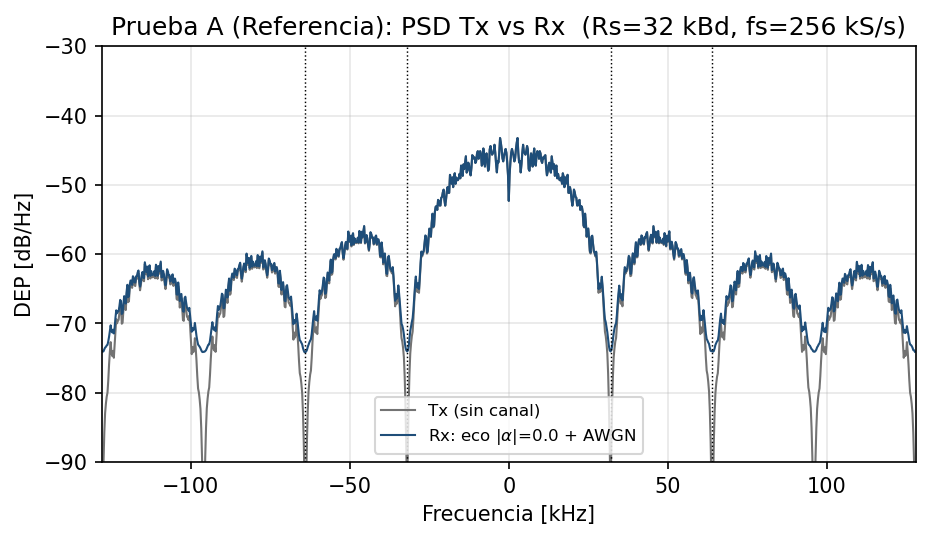
\includegraphics[width=\columnwidth]{PSD_prueba_A.png}\\[-1pt]
{\scriptsize (a)}\\
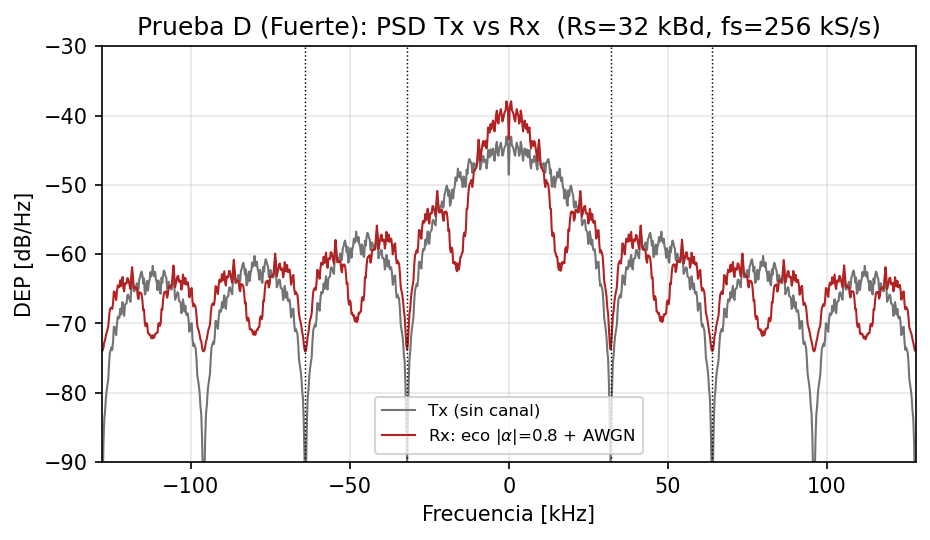
\includegraphics[width=\columnwidth]{PSD_prueba_D.png}\\[-1pt]
{\scriptsize (b)}
\caption{PSD Tx vs.\ Rx (Welch, 1024 puntos): (a) prueba A, referencia; (b) prueba D, $|\alpha|=0{,}8$.}
\label{fig:psd}
\end{figure}

\begin{figure}[!t]
\centering
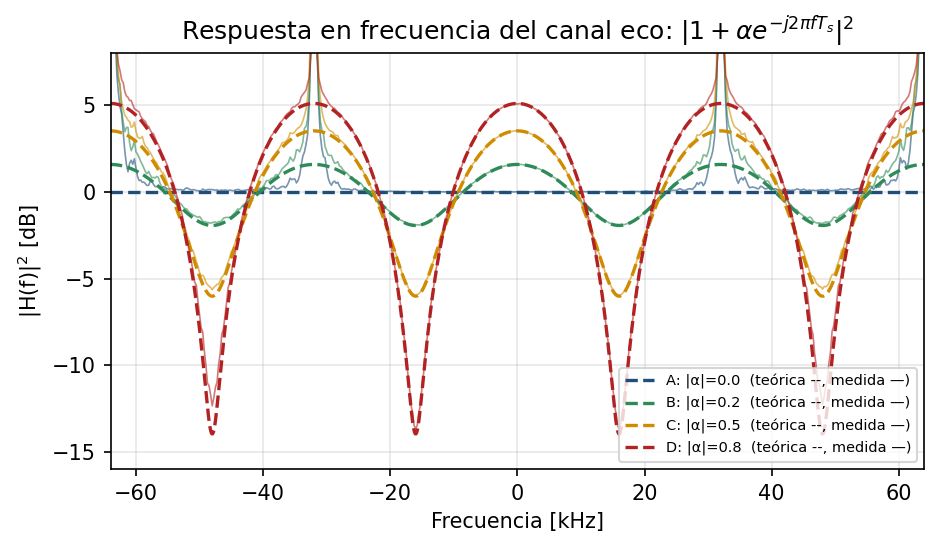
\includegraphics[width=\columnwidth]{Respuesta_frecuencia_canal.png}
\caption{Respuesta en frecuencia del canal: cociente medido $P_{rx}/P_{tx}$ (línea continua) frente al modelo $|1+\alpha e^{-j2\pi fT_s}|^2$ (línea discontinua).}
\label{fig:hf}
\end{figure}

\subsection{Señal temporal}
En la prueba C (Figura~\ref{fig:temporal}), cada símbolo de la señal recibida toma el valor $s_k+0{,}5\,s_{k-1}$. Cuando dos bits consecutivos son iguales el nivel sube a $\pm1{,}5$, y cuando cambian baja a $\pm0{,}5$. La salida del filtro acoplado integra cada símbolo y alcanza su valor final en la muestra $8k+7$ (puntos negros). Ese es el instante que selecciona \emph{Keep One in N}. El efecto del eco, por tanto, es visible en el tiempo: los niveles dependen del símbolo anterior, que es la definición de ISI.

\begin{figure}[!t]
\centering
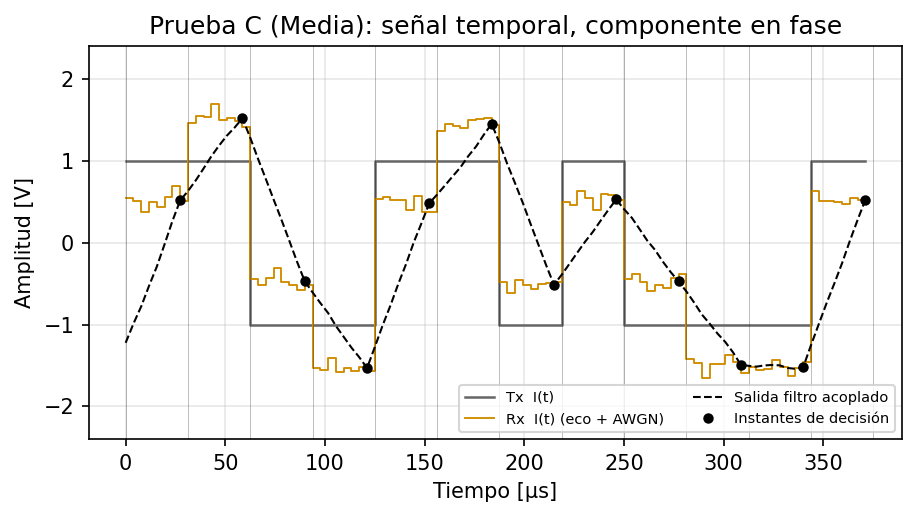
\includegraphics[width=\columnwidth]{Temporal_prueba_C.png}
\caption{Prueba C ($|\alpha|=0{,}5$): componente en fase Tx, Rx y salida del filtro acoplado con los instantes de decisión.}
\label{fig:temporal}
\end{figure}

\subsection{Constelación y diagrama de ojo}
Las Figuras~\ref{fig:const} y \ref{fig:ojo} muestran la evolución de las cuatro pruebas.
\textbf{A (referencia):} dos nubes compactas en $\pm1$ (EVM 3,5~\%) y un ojo abierto con apertura 1,84~V, limitada solo por el ruido. Es la línea base del receptor.
\textbf{B (suave):} cada nube se divide en dos, en $\pm1\pm0{,}2$, y el ojo baja a 1,46~V. La degradación comienza, pero el margen sigue siendo amplio, y el AWGN de referencia no produce errores.
\textbf{C (media):} los cuatro niveles $\pm0{,}5$ y $\pm1{,}5$ quedan bien separados. El ojo se reduce a la mitad (0,86~V), así que cualquier aumento del ruido se traduce rápidamente en errores. Esta es la condición principal de análisis porque muestra con claridad el mecanismo de ISI.
\textbf{D (fuerte):} los niveles internos $\pm0{,}2$ quedan a solo 0,2~V del umbral y el ojo casi se cierra (0,26~V). Con \texttt{noise\_amp}$=0{,}10$ todavía no hay errores, porque la desviación del ruido tras el filtro es $\approx0{,}025$~V, pero el sistema queda en estrés: la BER depende ahora casi por completo del margen residual $1-|\alpha|$.

Como resume la Figura~\ref{fig:apertura}, la apertura medida sigue la recta teórica $2(1-|\alpha|)$, desplazada unos 0,15~V por el ruido. Esto confirma la hipótesis: el eco no rota ni dispersa la constelación al azar, sino que la \emph{desdobla} de forma determinista según el símbolo anterior.

\begin{figure*}[!t]
\centering
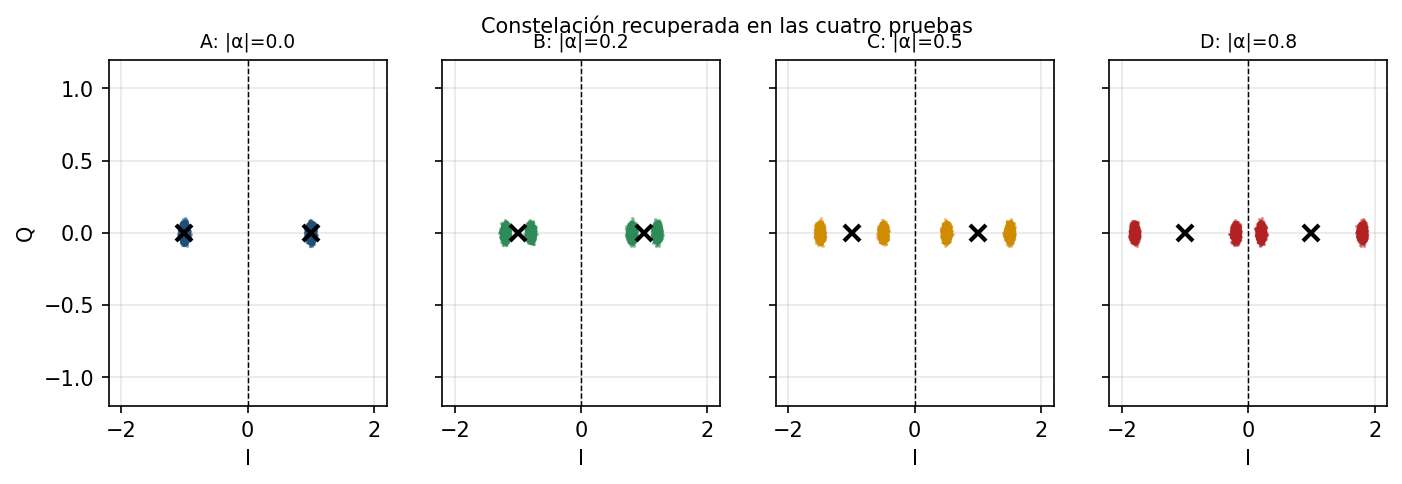
\includegraphics[width=0.9\textwidth]{Constelaciones_comparacion_ABCD.png}
\caption{Constelación recuperada (1 muestra/símbolo) en las pruebas A--D. Las cruces son los símbolos ideales $\pm1$.}
\label{fig:const}
\end{figure*}

\begin{figure*}[!t]
\centering
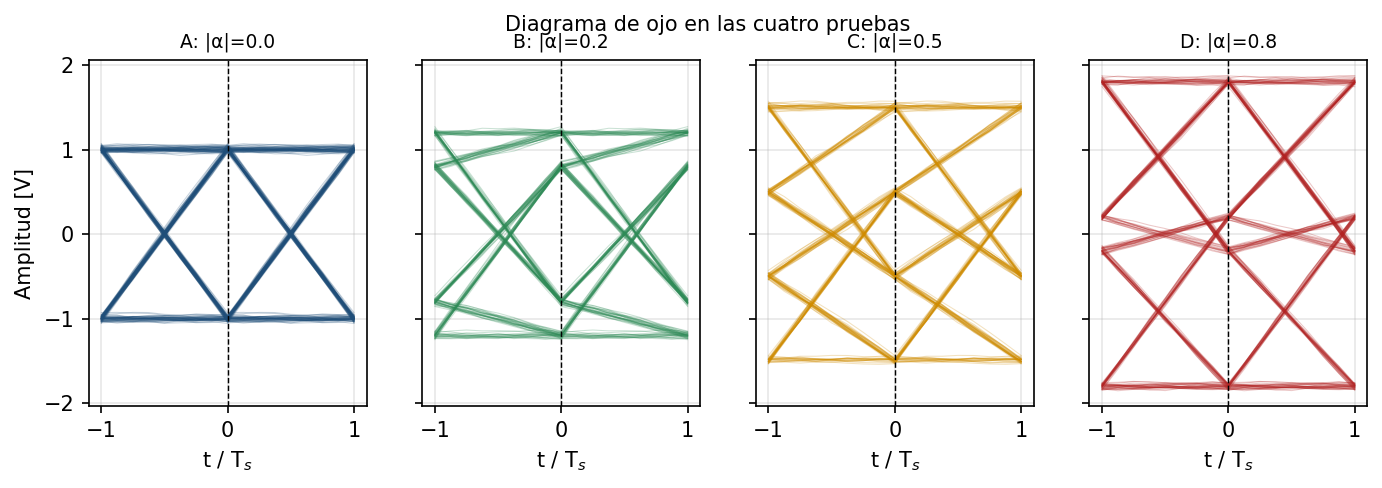
\includegraphics[width=0.9\textwidth]{Ojos_comparacion_ABCD.png}
\caption{Diagrama de ojo a la salida del filtro acoplado (parte real) en las pruebas A--D; $t=0$ es el instante de decisión.}
\label{fig:ojo}
\end{figure*}

\begin{figure}[!t]
\centering
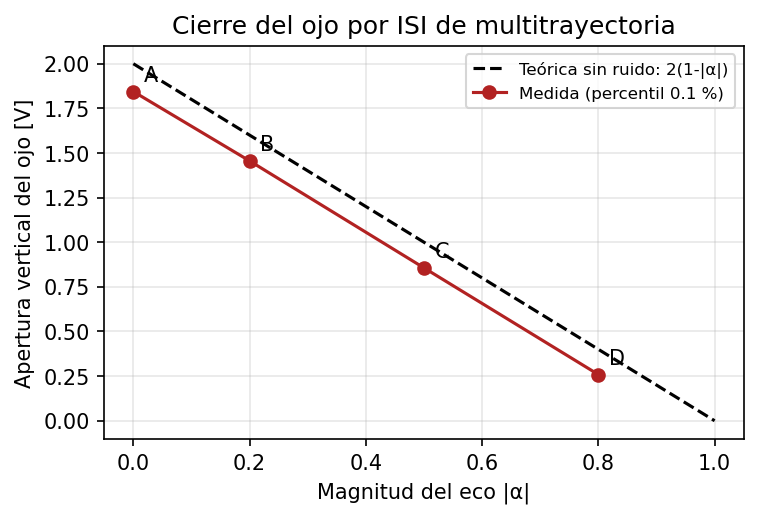
\includegraphics[width=0.85\columnwidth]{Apertura_ojo_vs_alpha.png}
\caption{Apertura vertical del ojo medida frente a la teórica sin ruido $2(1-|\alpha|)$.}
\label{fig:apertura}
\end{figure}

\subsection{Curva BER vs.\ $E_b/N_0$}
La Figura~\ref{fig:ber} presenta las curvas obtenidas directamente de los archivos \texttt{curva\_BER.csv} generados por el instrumento, sin editar. Para $\alpha=0$, la BER medida sigue $Q(\sqrt{2E_b/N_0})$: $7{,}9\times10^{-2}$ a 0~dB (teoría $7{,}9\times10^{-2}$), $8{,}1\times10^{-4}$ a 7~dB (teoría $7{,}7\times10^{-4}$) y $3{,}5\times10^{-5}$ a 9~dB. A partir de 10~dB no se detectaron errores en 200\,000 bits por punto. Esto no significa BER $=0$: indica $BER<1{,}5\times10^{-5}$, que el instrumento grafica como la cota $3/N$. Una ejecución independiente en el equipo del grupo (GRC 3.10.12, Windows) reprodujo la curva con diferencias dentro de la dispersión estadística (p.~ej., $7{,}2\times10^{-4}$ a 7~dB).

Con eco, las curvas se desplazan a la derecha y se aplanan, en concordancia con \eqref{eq:pb} (Tabla~\ref{tab:penalizacion}). El término $(1-|\alpha|)$ domina la BER, y además el eco ``gasta'' energía: $E_b$ se mide sobre la potencia total $1+|\alpha|^2$, pero solo la parte coherente ayuda a la decisión. Según el criterio del proyecto (penalización $\le2$~dB a BER $=10^{-3}$), el eco suave es tolerable sin ecualización (1,4~dB), el eco medio no lo es (6,3~dB) y con el eco fuerte la curva no alcanza $10^{-3}$ en todo el barrido. La teoría predice 22,3~dB, es decir, una penalización de unos 15,5~dB. Las diferencias entre medición y teoría están dentro de $\pm0{,}05$~dB, lo que valida tanto la integración del instrumento como la alineación \texttt{delay\_bits}$=0$.

\begin{figure}[!t]
\centering
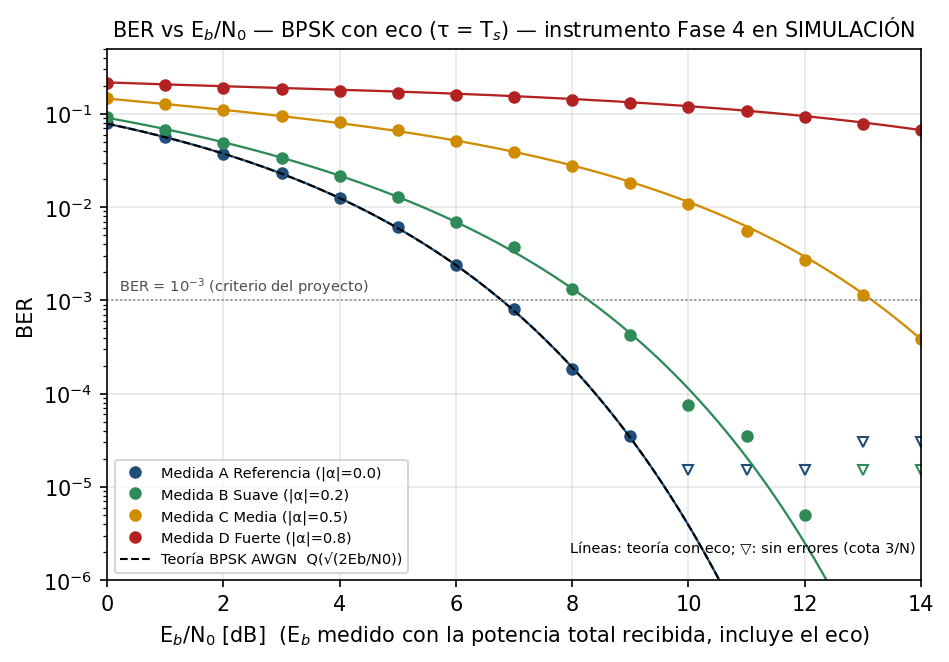
\includegraphics[width=\columnwidth]{BER_vs_EbN0_eco.png}
\caption{BER vs.\ $E_b/N_0$ medida con el instrumento de la Fase~4 (simulación) para las cuatro pruebas, con la teoría de \eqref{eq:pb} y la curva BPSK en AWGN.}
\label{fig:ber}
\end{figure}

\begin{table}[!t]
\centering
\caption{$E_b/N_0$ requerido para BER $=10^{-3}$ y penalización por eco}
\label{tab:penalizacion}
\footnotesize
\begin{tabular}{lcccc}
\toprule
$|\alpha|$ & \textbf{Medido} [dB] & \textbf{Teórico} [dB] & \textbf{Penalización} [dB] & \textbf{$\le$2 dB} \\
\midrule
0   & 6,80 & 6,79 & 0 (ref.) & Sí \\
0,2 & 8,24 & 8,28 & 1,44 & Sí \\
0,5 & 13,11 & 13,16 & 6,31 & No \\
0,8 & $>14$ & 22,3 & $\approx15{,}5$ (teórica) & No \\
\bottomrule
\end{tabular}
\end{table}

\subsection{Observaciones de la verificación}
(i) En GRC~3.10.12 (Windows), el \emph{QT GUI Vector Sink} de la plantilla no redibujó la curva durante la ejecución, aunque el bloque CSV, conectado a la misma salida, guardó correctamente los valores. Por ello se tomó como evidencia el CSV, que es el archivo que exige la guía. (ii) La fuente de bits del curso repite una secuencia de 1000 bits, lo que introduce una pequeña correlación $\rho_1$ entre símbolos y explica las variaciones de potencia recibida entre ejecuciones. (iii) El modelo considera un único eco con fase $0^\circ$, el peor caso en fase. Con otra fase, parte del eco cae en la componente Q, y en BPSK el ojo del eje I se cierra solo en $|\alpha|\cos\varphi$.
